\documentclass[a4paper,14pt]{extreport} % формат документа

\usepackage{amsmath}
\usepackage{cmap} % поиск в ПДФ
\usepackage[T2A]{fontenc} % кодировка
\usepackage[utf8]{inputenc} % кодировка исходного текста
\usepackage[english,russian]{babel} % локализация и переносы
\usepackage[left = 2cm, right = 1cm, top = 2cm, bottom = 2 cm]{geometry} % поля
\usepackage{listings}
\usepackage{graphicx} % для вставки рисунков
\usepackage{amsmath}
\usepackage{float}
\usepackage{longtable}
\usepackage{multirow}
\graphicspath{{pictures/}}
\DeclareGraphicsExtensions{.pdf,.png,.jpg}
\newcommand{\anonsection}[1]{\section*{#1}\addcontentsline{toc}{section}{#1}}

\lstset{ %
	language=Prolog,                % Язык программирования 
	numbers=left,                   % С какой стороны нумеровать          
	frame=single,                    % Добавить рамку
}

\begin{document}
\begin{titlepage}

    \begin{table}[H]
        \centering
        \footnotesize
        \begin{tabular}{cc}
            \multirow{8}{*}{
\includegraphics[scale=0.35]{bmstu.jpg}}
            & \\
            & \\
            & \textbf{Министерство науки и высшего образования Российской Федерации} \\
            & \textbf{Федеральное государственное бюджетное образовательное учреждение} \\
            & \textbf{высшего образования} \\
            & \textbf{<<Московский государственный технический} \\
            & \textbf{университет имени Н.Э. Баумана>>} \\
            & \textbf{(МГТУ им. Н.Э. Баумана)} \\
        \end{tabular}
    \end{table}

    \vspace{-2.5cm}

    \begin{flushleft}
        \rule[-1cm]{\textwidth}{3pt}
        \rule{\textwidth}{1pt}
    \end{flushleft}

    \begin{flushleft}
        \small
        ФАКУЛЬТЕТ
        \underline{<<Информатика и системы управления>>\ \ \ \ \ \ \ 
        \ \ \ \ \ \ \ \ \ \ \ \ \ \ \ \ \ \ \ \ \ \ \ \ \ \ \ \ \ \ \ 
    \ \ \ \ \ \ \ \ \ \ \ \ \ \ \ } \\
        КАФЕДРА
        \underline{<<Программное обеспечение ЭВМ и
        информационные технологии>>
        \ \ \ \ \ \ \ \ \ \ \ \ \ \ \ \ \ \ \ \ }
    \end{flushleft}

    \vspace{4cm}

    \begin{center}
        \textbf{Лабораторная работа № 13} \\ 
        \hfill
        
        \textbf{Работа программы на Prolog} \\
        \vspace{0.5cm}
        \textbf{} \\
    \end{center}

    \vspace{4cm}

    \begin{flushleft}
        \begin{tabular}{ll}
            \textbf{Дисциплина} & Функциональное и логическое программирование \\
            \textbf{Студент} & Сиденко А.Г. \\
            \textbf{Группа} & ИУ7-63Б \\
            \textbf{Преподаватель} & Толпинская Н.Б., Строганов Ю.В.  \\
        \end{tabular}
    \end{flushleft}

    \vspace{4cm}

   \begin{center}
        Москва, 2020 г.
    \end{center}

\end{titlepage}

\textbf{Задание}

Составить программу, т.е. модель предметной области – базу знаний, объединив в ней информацию – знания:

\begin{enumerate}
\item \textbf{<<Телефонный справочник>>}: Фамилия, №тел, Адрес – структура (Город, Улица, №дома, №кв),
\item \textbf{<<Автомобили>>}: Фамилия\_владельца, Марка, Цвет, Стоимость, и др.,
\item \textbf{<<Вкладчики банков>>}: Фамилия, Банк, счет, сумма, др.
\end{enumerate}

Владелец может иметь несколько телефонов, автомобилей, вкладов (Факты).

\hfill

Используя правила, обеспечить возможность поиска:

\begin{enumerate}
\item 
\begin{enumerate}
\item По № телефона найти: Фамилию, Марку автомобиля, Стоимость автомобиля (может быть несколько),
\item Используя сформированное в пункте а) правило, по № телефона найти: только Марку автомобиля (автомобилей может быть несколько),
\end{enumerate}
\item Используя простой, не составной вопрос: по Фамилии (уникальна в городе, но в разных городах есть однофамильцы) и Городу проживания найти:  Улицу проживания, Банки, в которых есть вклады и №телефона. 
\end{enumerate}

\textbf{Для задания1 и задания2: }

для одного из вариантов ответов, и для а) и для в), описать словесно порядок поиска ответа на вопрос, указав, как выбираются знания, и, при этом, для каждого этапа унификации, выписать подстановку – наибольший общий унификатор, и соответствующие примеры термов.

\hfill

\textbf{Программа}

\begin{lstlisting}
domains
  lastname, city, street, model, color, bank = symbol.
  telephone, house, flat, price, account, deposit = integer.
  adress = adress(city, street, house, flat).
predicates
  abonent(lastname, telephone, adress).
  auto(lastname, city, model, color, price).
  depositor(lastname, city, bank, account, deposit).
  
  autoByNumber(telephone, lastname, model, price).
  modelAutoByNumber(telephone, model).
  adressBankByLastnameCity(lastname,city,street,bank,telephone).
clauses
  abonent(ellen, 111111, adress(moscow, tverskaya, 1, 1)).
  abonent(john, 222222, adress(moscow, arbat, 11, 112)).
  abonent(tom, 333333, adress(moscow, presnya, 10, 11)).
  abonent(eric, 444444, adress(moscow, pokrovka, 21, 55)).
  abonent(mark, 555555, adress(moscow, solyanka, 13, 13)).
  abonent(mark, 888888, adress(kazan, pushkin, 22, 130)).
  abonent(bill, 666666, adress(ekb, lenin, 12, 88)).
  abonent(bill, 777777, adress(spb, sadovaya, 1, 12)).
  auto(ellen, moscow, bmw, red, 10000).
  auto(tom, moscow, mersedes, black, 15000).
  auto(eric, moscow, mersedes, white, 20000).
  auto(eric, moscow, bmw, black, 15000).
  auto(eric, moscow, porshe, red, 30000).
  auto(mark, moscow, hyundai, silver, 7000).
  auto(bill, ekb, hyundai, black, 10000).
  auto(bill, spb, volvo, black, 13000).
  depositor(ellen, moscow, sberbank, 10000, 2000).
  depositor(john, moscow, sberbank, 10000, 3000).
  depositor(john, moscow, vtb, 20000, 5000).
  depositor(eric, moscow, sberbank, 100000, 30000).
  depositor(mark, moscow, sberbank, 10000, 2000).
  depositor(mark, kazan, vtb, 10000, 2000).
  depositor(mark, moscow, gazprom, 10000, 2000).
  depositor(bill, spb, vtb, 30000, 3000).
  
  autoByNumber(Number, Name, Model, Price) :- 
    abonent(Name, Number, adress(City, _, _, _)),
    auto(Name, City, Model, _, Price).
    
  modelAutoByNumber(Number, Model) :-
    autoByNumber(Number, _, Model, _).
    
  adressBankByLastnameCity(Name, City, Street, Bank, Number):-
    abonent(Name, Number, adress(City, Street, _, _)),
    depositor(Name, City, Bank, _, _).
\end{lstlisting}

\begin{enumerate}
\item Задание 1
\begin{enumerate}
\item По № телефона найти: Фамилию, Марку автомобиля, Стоимость автомобиля


\begin{lstlisting}[caption=Пример 1 задание 1a]
goal
  Number = 444444,
  autoByNumber(Number, Name, Model, Price).
\end{lstlisting}


\includegraphics[scale=0.8]{ex1}

\begin{lstlisting}[caption=Пример 2 задание 1a]
goal
  Number = 666666,
  autoByNumber(Number, Name, Model, Price).
\end{lstlisting}

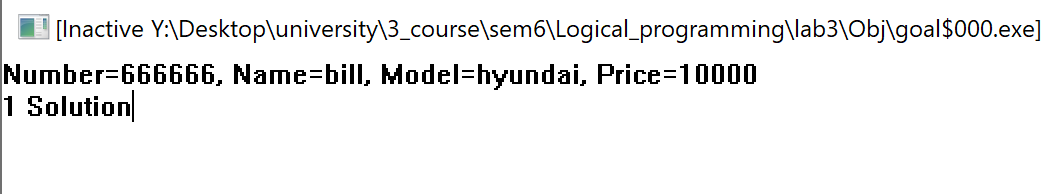
\includegraphics[scale=0.8]{ex2}


\begin{lstlisting}[caption=Пример 3 задание 1a]
goal
  Number = 444444,
  autoByNumber(Number, Name, Model, Price).
\end{lstlisting}

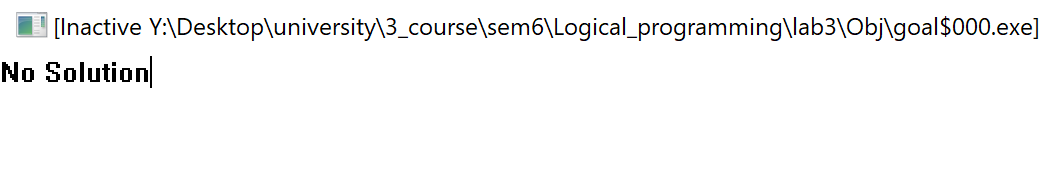
\includegraphics[scale=0.8]{ex3}

\textbf{Поиск ответа на вопрос из примера 2. }

\begin{longtable}{|p{1.1cm}|p{8.5cm}|p{7cm}|}
	\hline
 	№ шага & Сравниваемые термы; результат; подстановка, если есть  & Дальнейшие действия: прямой ход или откат \\ \hline
	1 & По autoByNumber(Number, Name, Model, Price) = autoByNumber(666666, Name, Model, Price) ищется системой определение отношения (по имени предиката и списку (числу) аргументов) & Определение отношения найдено, заносится в стек autoByNumber(666666, Name, Model, Price), прямой ход \\ \hline
	2 & Начинает <<раскрываться>> правило, т.е. доказывается каждое целевое утверждение в теле правила последовательно слева направо
	
	abonent(Name, Number, adress (City, \_, \_, \_)), auto(Name, City, Model, \_, Price) 
	
	& Заносится в стек abonent(Name, 666666, adress (City, \_, \_, \_)) \\ \hline
	
	3 & По abonent(Name, 666666, adress (City, \_, \_, \_)) ищется системой определение отношения (по имени предиката и списку (числу) аргументов) & Определение отношения найдено \\ \hline
	
	4 & Унификация abonent(ellen, 111111, adress (moscow, tverskaya, 1, 1)) с abonent(Name, 666666, adress (City, \_, \_, \_)) & Результат сравнения термов: false, переход к следующей строке (прямой ход) \\ \hline
	5 & Унификация abonent(john, 222222, adress(moscow, arbat, 11, 112)) с abonent(Name, 666666, adress (City, \_, \_, \_)) & Результат сравнения термов: false, переход к следующей строке (прямой ход) \\ \hline
	6 & Унификация abonent(tom, 333333, adress(moscow, presnya, 10, 11)) с abonent(Name, 666666, adress (City, \_, \_, \_)) & Результат сравнения термов: false, переход к следующей строке (прямой ход) \\ \hline
	7 & Унификация abonent(eric, 444444, adress(moscow, pokrovka, 21, 55)) с abonent(Name, 666666, adress (City, \_, \_, \_)) & Результат сравнения термов: false, переход к следующей строке (прямой ход) \\ \hline
	8 & Унификация abonent(mark, 555555, adress(moscow, solyanka, 13, 13)) с abonent(Name, 666666, adress (City, \_, \_, \_)) & Результат сравнения термов: false, переход к следующей строке (прямой ход) \\ \hline
	9 & Унификация abonent(mark, 888888, adress(kazan, pushkin, 22, 130)) с abonent(Name, 666666, adress (City, \_, \_, \_)) & Результат сравнения термов: false, переход к следующей строке (прямой ход) \\ \hline
	10 & Унификация abonent(bill, 666666, adress(ekb, lenin, 12, 88)) с abonent(Name, 666666, adress (City, \_, \_, \_)) & Результат сравнения термов: true, Name примет значение bill, City примет значение ekb. Установим маркер.  Анонимные переменные не связываются со значением. Переход к следующему целевому утверждению в теле правила (прямой ход) \\ \hline
	11 & Следующее целевое утверждение auto(Name, City, Model, \_, Price) & Заносится в стек auto(bill, ekb, Model, \_, Price)  \\ \hline
	12 & По auto(bill, ekb, Model, \_, Price) ищется системой определение отношения (по имени предиката и списку (числу) аргументов) & Определение отношения найдено \\ \hline
	13 & Унификация auto(ellen, moscow, bmw, red, 10000) с auto(bill, ekb, Model, \_, Price) & Результат сравнения термов: false, переход к следующей строке (прямой ход) \\ \hline
	14 & Унификация auto(tom, moscow, mersedes, black, 15000) с auto(bill, ekb, Model, \_, Price) & Результат сравнения термов: false, переход к следующей строке (прямой ход) \\ \hline
	15 & Унификация auto(eric, moscow, mersedes, white, 20000) с auto(bill, ekb, Model, \_, Price) & Результат сравнения термов: false, переход к следующей строке (прямой ход) \\ \hline
	16 & Унификация auto(eric, moscow, bmw, black, 15000) с auto(bill, ekb, Model, \_, Price) & Результат сравнения термов: false, переход к следующей строке (прямой ход) \\ \hline
	17 & Унификация auto(eric, moscow, porshe, red, 30000) с auto(bill, ekb, Model, \_, Price) & Результат сравнения термов: false, переход к следующей строке (прямой ход) \\ \hline
	18 & Унификация auto(mark, moscow, hyundai, silver, 7000) с auto(bill, ekb, Model, \_, Price) & Результат сравнения термов: false, переход к следующей строке (прямой ход) \\ \hline
	19 & Унификация auto(bill, ekb, hyundai, black, 10000) с auto(bill, ekb, Model, \_, Price) & Результат сравнения термов: true, вывод результата, переход к следующей строке (прямой ход) \\ \hline
	20 & Унификация auto(bill, spb, volvo, black, 13000) с auto(bill, ekb, Model, \_, Price) & Результат сравнения термов: false, в базе знаний больше ни одного утверждения с заданным именем, возврат, достаем из стека auto(bill, ekb, Model, \_, Price) \\ \hline
	21 & Унификация abonent(bill, 777777, adress(spb, sadovaya, 1, 12)) с abonent(Name, 666666, adress (City, \_, \_, \_)) & Результат сравнения термов: false, в базе знаний больше ни одного утверждения с заданным именем, возврат, достаем из стека abonent(Name, 666666, adress (City, \_, \_, \_)) \\ \hline
	22 & Достаем из стека autoByNumber(666666, Name, Model, Price) & Стек пуст, завершение программы \\ \hline
\end{longtable}

\item По № телефона найти: Марку автомобиля

\begin{lstlisting}[caption=Пример 1 задание 1b]
goal
  Number = 666666,
  modelAutoByNumber(Number, Model).
\end{lstlisting}

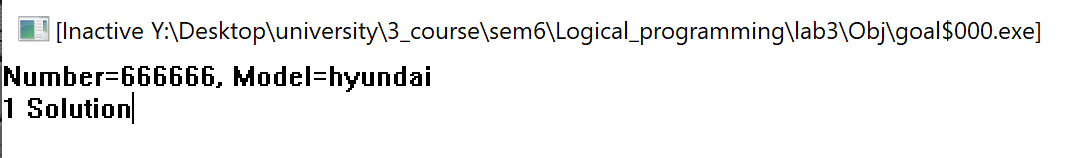
\includegraphics[scale=0.8]{ex4}

\begin{lstlisting}[caption=Пример 2 задание 1b]
goal
  Number = 222222,
  modelAutoByNumber(Number, Model).
\end{lstlisting}

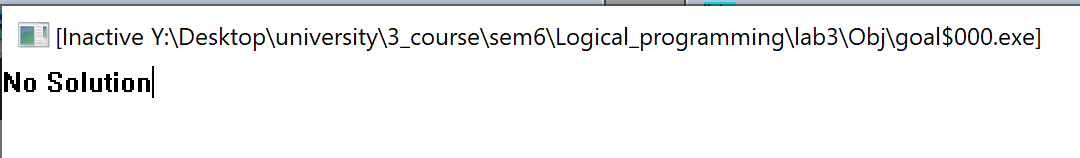
\includegraphics[scale=0.8]{ex5}

\begin{lstlisting}[caption=Пример 3 задание 1b]
goal
  Number = 111111,
  modelAutoByNumber(Number, Model).
\end{lstlisting}

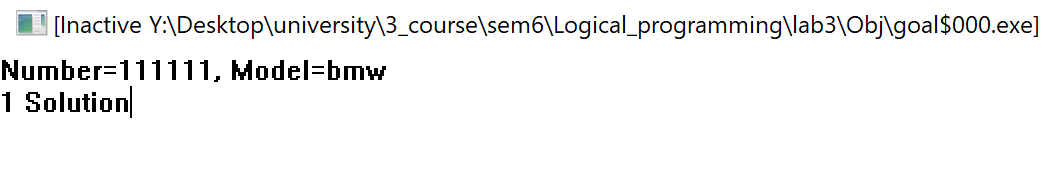
\includegraphics[scale=0.8]{ex6}

\end{enumerate}

\textbf{Поиск ответа на вопрос из примера 3. }

\begin{longtable}{|p{1.1cm}|p{8.5cm}|p{7cm}|}
	\hline
 	№ шага & Сравниваемые термы; результат; подстановка, если есть  & Дальнейшие действия: прямой ход или откат \\ \hline
	1 & По modelAutoByNumber(Number, Model) = modelAutoByNumber(111111, Model) ищется системой определение отношения (по имени предиката и списку (числу) аргументов) & Определение отношения найдено, заносится в стек modelAutoByNumber(111111, Model), прямой ход \\ \hline
	2 & Начинает <<раскрываться>> правило, т.е. доказывается каждое целевое утверждение в теле правила последовательно слева направо autoByNumber(Number, \_, Model, \_)
	& Заносится в стек autoByNumber(111111, \_, Model, \_), прямой ход \\ \hline
	3 & По autoByNumber(111111, \_, Model, \_) ищется системой определение отношения (по имени предиката и списку (числу) аргументов) & Определение отношения найдено \\ \hline
	4 & Начинает <<раскрываться>> правило, т.е. доказывается каждое целевое утверждение в теле правила последовательно слева направо abonent(Name, Number, adress (City, \_, \_, \_)), auto(Name, City, Model, \_, \_)
	& Заносится в стек abonent(Name, 111111, adress (City, \_, \_, \_)), прямой ход \\ \hline
	5 & По abonent(Name, 111111, adress (City, \_, \_, \_)) ищется системой определение отношения (по имени предиката и списку (числу) аргументов) & Определение отношения найдено \\ \hline
	6 & Унификация abonent(ellen, 111111, adress (moscow, tverskaya, 1, 1)) с abonent(Name, 111111, adress (City, \_, \_, \_)) & Результат сравнения термов: true, Name примет значение ellen, City примет значение moscow. Установим маркер. Анонимные переменные не связываются со значением. Переход к следующему целевому утверждению в теле правила (прямой ход) \\ \hline
	7 & Следующее целевое утверждение auto(Name, City, Model, \_, Price) & Заносится в стек auto(ellen, moscow, Model, \_, \_)  \\ \hline
	8 & По auto(ellen, moscow, Model, \_, \_) ищется системой определение отношения (по имени предиката и списку (числу) аргументов) & Определение отношения найдено \\ \hline
	9 & Унификация auto(ellen, moscow, bmw, red, 10000) с auto(ellen, moscow, Model, \_, \_) & Результат сравнения термов: true, вывод результата, переход к следующей строке (прямой ход) \\ \hline
	10 & Унификация auto(tom, moscow, mersedes, black, 15000) с auto(ellen, moscow, Model, \_, \_) & Результат сравнения термов: false, переход к следующей строке (прямой ход) \\ \hline
	11 & Унификация auto(eric, moscow, mersedes, white, 20000) с auto(ellen, moscow, Model, \_, \_) & Результат сравнения термов: false, переход к следующей строке (прямой ход) \\ \hline
	12 & Унификация auto(eric, moscow, bmw, black, 15000) с auto(ellen, moscow, Model, \_, \_) & Результат сравнения термов: false, переход к следующей строке (прямой ход) \\ \hline
	13 & Унификация auto(eric, moscow, porshe, red, 30000) с auto(ellen, moscow, Model, \_, \_) & Результат сравнения термов: false, переход к следующей строке (прямой ход) \\ \hline
	14 & Унификация auto(mark, moscow, hyundai, silver, 7000) с auto(ellen, moscow, Model, \_, \_) & Результат сравнения термов: false, переход к следующей строке (прямой ход) \\ \hline
	15 & Унификация auto(bill, ekb, hyundai, black, 10000) с auto(ellen, moscow, Model, \_, \_) & Результат сравнения термов: false, переход к следующей строке (прямой ход) \\ \hline
	16 & Унификация auto(bill, spb, volvo, black, 13000) с auto(ellen, moscow, Model, \_, \_) & Результат сравнения термов: false, в базе знаний больше ни одного утверждения с заданным именем, возврат, достаем из стека auto(bill, ekb, Model, \_, \_) \\ \hline

	17 & Унификация abonent(john, 222222, adress(moscow, arbat, 11, 112)) с abonent(Name, 111111, adress (City, \_, \_, \_)) & Результат сравнения термов: false, переход к следующей строке (прямой ход) \\ \hline
	18 & Унификация abonent(tom, 333333, adress(moscow, presnya, 10, 11)) с abonent(Name, 111111, adress (City, \_, \_, \_)) & Результат сравнения термов: false, переход к следующей строке (прямой ход) \\ \hline
	19 & Унификация abonent(eric, 444444, adress(moscow, pokrovka, 21, 55)) с abonent(Name, 111111, adress (City, \_, \_, \_)) & Результат сравнения термов: false, переход к следующей строке (прямой ход) \\ \hline
	20 & Унификация abonent(mark, 555555, adress(moscow, solyanka, 13, 13)) с abonent(Name, 111111, adress (City, \_, \_, \_)) & Результат сравнения термов: false, переход к следующей строке (прямой ход) \\ \hline
	21 & Унификация abonent(mark, 888888, adress(kazan, pushkin, 22, 130)) с abonent(Name, 111111, adress (City, \_, \_, \_)) & Результат сравнения термов: false, переход к следующей строке (прямой ход) \\ \hline
	22 & Унификация abonent(bill, 666666, adress(ekb, lenin, 12, 88)) с abonent(Name, 111111, adress (City, \_, \_, \_)) & Результат сравнения термов: true, Name примет значение bill, City примет значение ekb. Установим маркер.  Анонимные переменные не связываются со значением. Переход к следующему целевому утверждению в теле правила (прямой ход) \\ \hline
	23 & Унификация abonent(bill, 777777, adress(spb, sadovaya, 1, 12)) с abonent(Name, 111111, adress (City, \_, \_, \_)) & Результат сравнения термов: false, в базе знаний больше ни одного утверждения с заданным именем, возврат, достаем из стека abonent(Name, 111111, adress (City, \_, \_, \_)), откат \\ \hline
	24 & Достаем из стека autoByNumber(111111, \_, Model, \_) & Откат, больше нет целевых утверждений \\ \hline
	25 & Достаем из стека modelAutoByNumber(111111, Model) & Откат, стек пуст, завершение программы \\ \hline
\end{longtable}

\item По Фамилии и Городу проживания найти:  Улицу проживания, Банки, в которых есть вклады и №телефона.

\begin{lstlisting}[caption=Пример 1 задание 2]
goal
  Name = mark,
  City = moscow,
  adressBankByLastnameCity(Name,City,Street,Bank,Number).
\end{lstlisting}

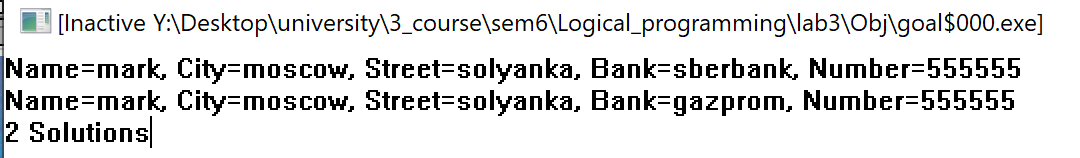
\includegraphics[scale=0.8]{ex7}

\begin{lstlisting}[caption=Пример 2 задание 2]
goal
  Name = mark,
  City = kazan,
  adressBankByLastnameCity(Name,City,Street,Bank,Number).
\end{lstlisting}

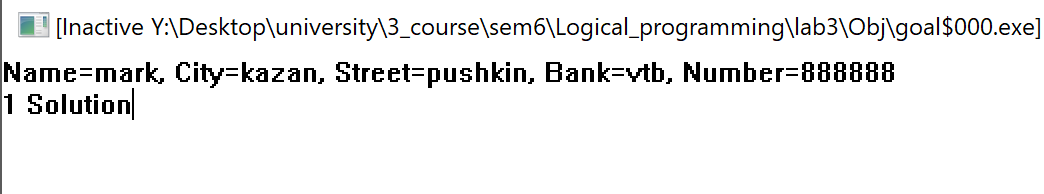
\includegraphics[scale=0.8]{ex8}

\begin{lstlisting}[caption=Пример 3 задание 2]
goal
  Name = mark,
  City = spb,
  adressBankByLastnameCity(Name,City,Street,Bank,Number).
\end{lstlisting}

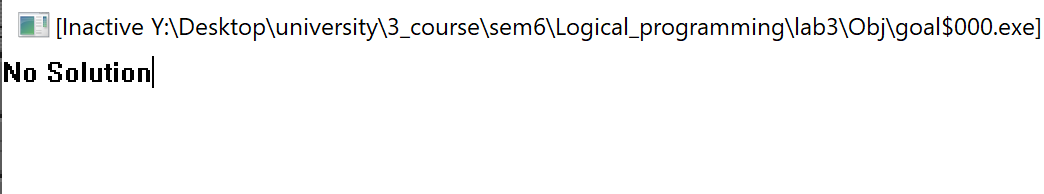
\includegraphics[scale=0.8]{ex9}

\end{enumerate}

\textbf{Поиск ответа на вопрос из примера 2. }

\begin{longtable}{|p{1.1cm}|p{8.5cm}|p{7cm}|}
	\hline
 	№ шага & Сравниваемые термы; результат; подстановка, если есть  & Дальнейшие действия: прямой ход или откат \\ \hline
	1 & По adressBankByLastnameCity(Name, City, Street, Bank, Number) = adressBankByLastnameCity(mark, kazan, Street, Bank, Number) ищется системой определение отношения (по имени предиката и списку (числу) аргументов) & Определение отношения найдено, заносится в стек adressBankByLastnameCity(mark, kazan, Street, Bank, Number), прямой ход \\ \hline
	2 & Начинает <<раскрываться>> правило, т.е. доказывается каждое целевое утверждение в теле правила последовательно слева направо
	abonent(Name, Number, adress(City, Street, \_, \_)), depositor(Name, City, Bank, \_, \_) 
	
	& Заносится в стек abonent(mark, Number, adress(kazan, Street, \_, \_)) \\ \hline
	
	3 & По abonent(mark, Number, adress(kazan, Street, \_, \_))  ищется системой определение отношения (по имени предиката и списку (числу) аргументов) & Определение отношения найдено \\ \hline
	
	4 & Унификация abonent(ellen, 111111, adress (moscow, tverskaya, 1, 1)) с abonent(mark, Number, adress(kazan, Street, \_, \_)) & Результат сравнения термов: false, переход к следующей строке (прямой ход) \\ \hline
	5 & Унификация abonent(john, 222222, adress(moscow, arbat, 11, 112)) с abonent(mark, Number, adress(kazan, Street, \_, \_)) & Результат сравнения термов: false, переход к следующей строке (прямой ход) \\ \hline
	6 & Унификация abonent(tom, 333333, adress(moscow, presnya, 10, 11)) с abonent(mark, Number, adress(kazan, Street, \_, \_)) & Результат сравнения термов: false, переход к следующей строке (прямой ход) \\ \hline
	7 & Унификация abonent(eric, 444444, adress(moscow, pokrovka, 21, 55)) с abonent(mark, Number, adress(kazan, Street, \_, \_)) & Результат сравнения термов: false, переход к следующей строке (прямой ход) \\ \hline
	8 & Унификация abonent(mark, 555555, adress(moscow, solyanka, 13, 13)) с abonent(mark, Number, adress(kazan, Street, \_, \_))& Результат сравнения термов: false, переход к следующей строке (прямой ход) \\ \hline
	9 & Унификация abonent(mark, 888888, adress(kazan, pushkin, 22, 130)) с abonent(mark, Number, adress(kazan, Street, \_, \_))& Результат сравнения термов: true, Number примет значение 888888, Street примет значение pushkin. Установим маркер.  Анонимные переменные не связываются со значением. Переход к следующему целевому утверждению в теле правила (прямой ход) \\ \hline
	11 & Следующее целевое утверждение depositor(Name, City, Bank, \_, \_) & Заносится в стек depositor(mark, kazan, Bank, \_, \_)   \\ \hline
	12 & По depositor(mark, kazan, Bank, \_, \_) ищется системой определение отношения (по имени предиката и списку (числу) аргументов) & Определение отношения найдено \\ \hline
	13 & Унификация depositor(ellen, moscow, sberbank, 10000, 2000) с depositor(mark, kazan, Bank, \_, \_) & Результат сравнения термов: false, переход к следующей строке (прямой ход) \\ \hline
	14 & Унификация depositor(john, moscow, sberbank, 10000, 3000) с depositor(mark, kazan, Bank, \_, \_) & Результат сравнения термов: false, переход к следующей строке (прямой ход) \\ \hline
	15 & Унификация depositor(john, moscow, vtb, 20000, 5000) с depositor(mark, kazan, Bank, \_, \_) & Результат сравнения термов: false, переход к следующей строке (прямой ход) \\ \hline
	16 & Унификация depositor(eric, moscow, sberbank, 100000, 30000) с depositor(mark, kazan, Bank, \_, \_) & Результат сравнения термов: false, переход к следующей строке (прямой ход) \\ \hline
	17 & Унификация depositor(mark, moscow, sberbank, 10000, 2000 с depositor(mark, kazan, Bank, \_, \_) & Результат сравнения термов: false, переход к следующей строке (прямой ход) \\ \hline
	18 & Унификация depositor(mark, kazan, vtb, 10000, 2000) с depositor(mark, kazan, Bank, \_, \_) & Результат сравнения термов:  true, вывод результата, переход к следующей строке (прямой ход)\\ \hline
	19 & Унификация depositor(mark, moscow, gazprom, 10000, 2000) с depositor(mark, kazan, Bank, \_, \_) & Результат сравнения термов: false, переход к следующей строке (прямой ход) \\ \hline
	20 & Унификация depositor(bill, spb, vtb, 30000, 3000) с depositor(mark, kazan, Bank, \_, \_) & Результат сравнения термов: false, в базе знаний больше ни одного утверждения с заданным именем, возврат, достаем из стека depositor(mark, kazan, Bank, \_, \_) \\ \hline

	10 & Унификация abonent(bill, 666666, adress(ekb, lenin, 12, 88)) с abonent(mark, Number, adress(kazan, Street, \_, \_))& Результат сравнения термов: false, переход к следующей строке (прямой ход)\\ \hline
	21 & Унификация abonent(bill, 777777, adress(spb, sadovaya, 1, 12)) с abonent(mark, Number, adress(kazan, Street, \_, \_)) & Результат сравнения термов: false, в базе знаний больше ни одного утверждения с заданным именем, возврат, достаем из стека abonent(mark, Number, adress(kazan, Street, \_, \_)) \\ \hline
	22 & Достаем из стека adressBankByLastnameCity(mark, kazan, Street, Bank, Number) & Стек пуст, завершение программы \\ \hline
\end{longtable}

\hfill

\textbf{Ответы на вопросы}

\begin{enumerate}
\item Что такое терм?

\textbf{Термом} будем называть выражение, образованное из переменных и констант, возможно, с применением функций, а точнее:
\begin{enumerate}
\item всякая переменная или константа есть терм;
\item если t1,...,tn — термы, а f — n-местный функциональный символ,
то f(t1,...,tn) — терм;
\item других термов нет.

\end{enumerate}
\item Что такое предикат в матлогике (математике)?

\textbf{Предикатом} называется функция нескольких переменных, которая в области задания этих переменных, может принимать лишь два значения 1 или 0 (которые мы как всегда можем рассматривать как истину или ложь).
Если предикат зависит от п переменных, то он называется п-местным.

\item Что описывает предикат в Prolog?

Утверждения программы — это предикаты. 

\item Назовите виды предложений в программе и приведите примеры таких предложений из Вашей программы. Какие предложения являются основными, а какие – не основными?  Каковы: синтаксис и семантика (формальный смысл) этих предложений (основных и неосновных)?

\textbf{Предложения бывают двух видов}: факты и правила. 

Предложение более общего вида -- \textbf{правило} имеет вид:
	A :- B1,... , Bn. 

A называется заголовком правила, а B1,..., Bn -- телом правила.

\textbf{Факт} -- это частный случай правила. Факт -- это предложение, в котором отсутствует тело (т.е. тело пустое). 

Пример предложения:
\begin{lstlisting}
autoByNumber(Number, Name, Model, Price) :- 
  abonent(Name, Number, adress(City, _, _, _)),
  auto(Name, City, Model, _, Price).
\end{lstlisting}

Пример факта:
\begin{lstlisting}
abonent(ellen, 111111, adress(moscow, tverskaya, 1, 1)).
\end{lstlisting}

\item Каковы назначение, виды и особенности использования переменных в программе на Prolog? Какое предложение БЗ сформулировано в более общей – абстрактной форме: содержащее или не содержащее переменных?

При поступлении вопроса с переменной в Пролог-систему. Например:
\begin{lstlisting}
universe("Mark", X).
\end{lstlisting}

X -- переменная, входящая в вопрос, изначально является \textbf{неконкретизированной}. Пролог просматривает базу данных в поисках факта, сопоставимого с вопросом. Если неконкретизированная переменная появляется в качестве одного из аргументов, то Пролог считает, что такой аргумент сопоставим с любым другим аргументом, находящимся в том же факте. При обнаружении такого факта переменная X становится \textbf{конкретизированной}, обозначая объект, являющийся вторым аргументом найденного факта.

Это относится только к именованным переменным. \textbf{Анонимные переменные} не могут быть связаны со значением.

Если составные термы, факты, правила и вопросы не содержат переменных, то они называются основными. Составные термы, факты, правила и вопросы в момент фиксации в программе могут содержать переменные, тогда они называются неосновными. 

\item Что такое подстановка?

Пусть дан терм: $A(X_1, X_2,..., X_n)$

Подстановкой называется множество пар, вида: $\{X_i = t_i\}$, 
где $X_i$ -- переменная, а $t_i$ -- терм.

\item Что такое пример терма? Как и когда строится? Как Вы думаете, система строит и хранит примеры?

Пусть $\theta = \{ X_1 = t_1, X_2= t_2, … , X_n = t_n \}$ -- подстановка,  тогда результат применения подстановки к терму обозначается: $A\theta$. Применение подстановки заключается в замене каждого вхождения переменной $X_i$  на соответствующий терм. Терм $B$ называется \textbf{примером терма} $A$, если существует такая подстановка $\theta$, что $B=A\theta$.

В процессе выполнения программы -- система, используя встроенный алгоритм унификации, пытается обосновать возможность истинности вопроса, строя подстановки и примеры термов (вопроса и формулировки знания), используя базу знаний. 

 \end{enumerate}
 
\end{document}